\documentclass{article}

  % packages
    % basic stuff for rendering math
    \usepackage[letterpaper, top=1in, bottom=1in, left=1in, right=1in]{geometry}
    \usepackage[english]{babel}
    \usepackage{amsmath, amssymb} 
    \usepackage{bbm}              % for mathbbm

    % extra math symbols and utilities
    \usepackage{mathtools}        % for extra stuff like \coloneqq
    \usepackage{mathrsfs}         % for extra stuff like \mathsrc{}
    \usepackage{centernot}        % for the centernot arrow 
    \usepackage{bm}               % for better boldsymbol/mathbf 
    \usepackage{enumitem}         % better control over enumerate, itemize
    \usepackage{xr-hyper}
    \usepackage{hyperref}         % for hypertext linking
    \usepackage{fancyvrb}          % for better verbatim environments
    \usepackage{newverbs}         % for texttt{}
    \usepackage{xcolor}           % for colored text 
    \usepackage{listings}         % to include code
    \usepackage{lstautogobble}    % helper package for code
    \usepackage{parcolumns}       % for side by side columns for two column code
    

    % page layout
    \usepackage{fancyhdr}         % for headers and footers 
    \usepackage{lastpage}         % to include last page number in footer 
    \usepackage{parskip}          % for no indentation and space between paragraphs    
    \usepackage[T1]{fontenc}      % to include \textbackslash
    \usepackage{footnote}
    \usepackage{etoolbox}

    % for custom environments
    \usepackage{tcolorbox}        % for better colored boxes in custom environments
    \tcbuselibrary{breakable}     % to allow tcolorboxes to break across pages

    % figures and tables 
    \usepackage{pgfplots}
    \pgfplotsset{compat=1.18}
    \usepackage{float}            % for [H] figure placement
    \usepackage{tikz, tikz-cd}
    \usetikzlibrary{arrows, positioning, calc}
    \usepackage{graphicx}
    \usepackage{caption, subcaption} 
    \usepackage{dcolumn}

    \usepackage[nottoc]{tocbibind}
    \hfuzz=5.002pt                % ignore overfull hbox badness warnings below this limit

  % New and replaced operators
		\DeclareMathOperator{\id}{id}
		\DeclareMathOperator{\Ob}{Ob}
		\DeclareMathOperator{\Hom}{Hom}
		\DeclareMathOperator{\End}{End}
		\DeclareMathOperator{\Aut}{Aut}
		\DeclareMathOperator{\Mor}{Mor}
		\DeclareMathOperator{\Iso}{Iso}

		% Fundamental categories
		\DeclareMathOperator{\Set}{\mathbf{Set}}
		\DeclareMathOperator{\FinSet}{\mathbf{FinSet}}
		\DeclareMathOperator{\Rel}{\mathbf{Rel}}
		\DeclareMathOperator{\Cat}{\mathbf{Cat}}
		\DeclareMathOperator{\Grpd}{\mathbf{Grpd}}

		% Algebraic categories
		\DeclareMathOperator{\Group}{\mathbf{Grp}}
		\DeclareMathOperator{\Grp}{\mathbf{Grp}}
		\DeclareMathOperator{\Ab}{\mathbf{Ab}}
		\DeclareMathOperator{\Mon}{\mathbf{Mon}}
		\DeclareMathOperator{\SGrp}{\mathbf{SGrp}}
		\DeclareMathOperator{\Ring}{\mathbf{Ring}}
		\DeclareMathOperator{\CRing}{\mathbf{CRing}}
		\DeclareMathOperator{\Field}{\mathbf{Field}}
		\DeclareMathOperator{\Mod}{\mathbf{Mod}}
		\DeclareMathOperator{\Vect}{\mathbf{Vect}}
		\DeclareMathOperator{\FinVect}{\mathbf{FinVect}}
		\DeclareMathOperator{\Alg}{\mathbf{Alg}}
		\DeclareMathOperator{\LieAlg}{\mathbf{LieAlg}}
		\DeclareMathOperator{\Lat}{\mathbf{Lat}}
		\DeclareMathOperator{\BoolAlg}{\mathbf{BoolAlg}}

		% Order-theoretic categories
		\DeclareMathOperator{\Pos}{\mathbf{Pos}}
		\DeclareMathOperator{\PreOrd}{\mathbf{PreOrd}}
		\DeclareMathOperator{\Ord}{\mathbf{Ord}}
		\DeclareMathOperator{\CPO}{\mathbf{CPO}}

		% Topological categories
		\DeclareMathOperator{\Top}{\mathbf{Top}}
		\DeclareMathOperator{\Topstar}{\mathbf{Top}_*}
		\DeclareMathOperator{\Haus}{\mathbf{Haus}}
		\DeclareMathOperator{\CompHaus}{\mathbf{CompHaus}}
		\DeclareMathOperator{\Met}{\mathbf{Met}}
		\DeclareMathOperator{\Unif}{\mathbf{Unif}}
		\DeclareMathOperator{\HTop}{\mathbf{hTop}}
		\DeclareMathOperator{\CW}{\mathbf{CW}}

		% Geometric categories
		\DeclareMathOperator{\Man}{\mathbf{Man}}
		\DeclareMathOperator{\Diff}{\mathbf{Diff}}
		\DeclareMathOperator{\SmoothMan}{\mathbf{SmoothMan}}
		\DeclareMathOperator{\Riem}{\mathbf{Riem}}
		\DeclareMathOperator{\Symp}{\mathbf{Symp}}
		\DeclareMathOperator{\Sch}{\mathbf{Sch}}
		\DeclareMathOperator{\AffSch}{\mathbf{AffSch}}
		\DeclareMathOperator{\Var}{\mathbf{Var}}

		% Linear algebra and functional analysis
		\DeclareMathOperator{\Ban}{\mathbf{Ban}}
		\DeclareMathOperator{\Hilb}{\mathbf{Hilb}}
		\DeclareMathOperator{\Norm}{\mathbf{Norm}}
		\DeclareMathOperator{\TVS}{\mathbf{TVS}}
		\DeclareMathOperator{\HilbFin}{\mathbf{FinHilb}}

		% Homological algebra
		\DeclareMathOperator{\Ch}{\mathbf{Ch}}
		\DeclareMathOperator{\KCat}{\mathbf{K}}
		\DeclareMathOperator{\DCat}{\mathbf{D}}
		\DeclareMathOperator{\Sh}{\mathbf{Sh}}
		\DeclareMathOperator{\PSh}{\mathbf{PSh}}
		\DeclareMathOperator{\SAb}{\mathbf{sAb}}

		% Algebraic topology and homotopy theory
		\DeclareMathOperator{\sSet}{\mathbf{sSet}}
		\DeclareMathOperator{\Sp}{\mathbf{Sp}}
		\DeclareMathOperator{\Spectra}{\mathbf{Spectra}}

		% Probability and measure theory
		\DeclareMathOperator{\Meas}{\mathbf{Meas}}
		\DeclareMathOperator{\Prob}{\mathbf{Prob}}
		\DeclareMathOperator{\Stoch}{\mathbf{Stoch}}

		% Graphs and combinatorics
		\DeclareMathOperator{\Graph}{\mathbf{Graph}}
		\DeclareMathOperator{\Digraph}{\mathbf{Digraph}}
		\DeclareMathOperator{\SimpComp}{\mathbf{SimpComp}}

  % Custom Environments
    \tcbset{
      colframe = black,
      colback  = white,
      coltitle = black,
      colbacktitle = black!10,
      breakable, 
      arc=0mm,
      boxrule=1pt,
      left=8pt,
      right=8pt,
      top=6pt,
      bottom=6pt,
      before skip=12pt,
      after skip=12pt,
      bottomrule at break=-1pt,
      toprule at break=-1pt,
      fonttitle=\bfseries,
    }
    \newcounter{question}[section]
    \renewcommand{\thequestion}{\thesection.\arabic{question}}
    \NewDocumentEnvironment{question}{O{} o}{%
      \refstepcounter{question}%
      \ifstrempty{#1}{%
        \begin{tcolorbox}[title=\textbf{Question \thequestion}]%
      }{%
        \IfValueTF{#2}{%
          \begin{tcolorbox}[title=\textbf{Question \thequestion~(#1)}, label={#2}]%
        }{%
          \begin{tcolorbox}[title=\textbf{Question \thequestion~(#1)}]%
        }%
      }%
    }{%
      \end{tcolorbox}%
    }

    \newcounter{exercise}[section]
    \renewcommand{\theexercise}{\thesection.\arabic{exercise}}
    \NewDocumentEnvironment{exercise}{O{} o}{%
      \refstepcounter{exercise}%
      \ifstrempty{#1}{%
        \begin{tcolorbox}[title=\textbf{Exercise \theexercise}]%
      }{%
        \IfValueTF{#2}{%
          \begin{tcolorbox}[title=\textbf{Exercise \theexercise~(#1)}, label={#2}]%
        }{%
          \begin{tcolorbox}[title=\textbf{Exercise \theexercise~(#1)}]%
        }%
      }%
    }{%
      \end{tcolorbox}%
    }

    \newtcolorbox[auto counter, number within=section]{solution}[1][]
    {
      before skip = -7pt,
      before upper = \textit{Solution. },
    }

    \newcounter{theorem}[section]
    \renewcommand{\thetheorem}{\thesection.\arabic{theorem}}

    \NewDocumentEnvironment{lemma}{O{} o}{%
      \refstepcounter{theorem}%
      \ifstrempty{#1}{%
        \begin{tcolorbox}[title=\textbf{Lemma \thetheorem}]%
      }{%
        \IfValueTF{#2}{%
          \begin{tcolorbox}[title=\textbf{Lemma \thetheorem~(#1)}, label={#2}]%
        }{%
          \begin{tcolorbox}[title=\textbf{Lemma \thetheorem~(#1)}]%
        }%
      }%
    }{%
      \end{tcolorbox}%
    }

    \NewDocumentEnvironment{theorem}{O{} o}{%
      \refstepcounter{theorem}%
      \ifstrempty{#1}{%
        \begin{tcolorbox}[title=\textbf{Theorem \thetheorem}]%
      }{%
        \IfValueTF{#2}{%
          \begin{tcolorbox}[title=\textbf{Theorem \thetheorem~(#1)}, label={#2}]%
        }{%
          \begin{tcolorbox}[title=\textbf{Theorem \thetheorem~(#1)}]%
        }%
      }%
    }{%
      \end{tcolorbox}%
    }

    \NewDocumentEnvironment{corollary}{O{} o}{%
      \refstepcounter{theorem}%
      \ifstrempty{#1}{%
        \begin{tcolorbox}[title=\textbf{Corollary \thetheorem}]%
      }{%
        \IfValueTF{#2}{%
          \begin{tcolorbox}[title=\textbf{Corollary \thetheorem~(#1)}, label={#2}]%
        }{%
          \begin{tcolorbox}[title=\textbf{Corollary \thetheorem~(#1)}]%
        }%
      }%
    }{%
      \end{tcolorbox}%
    }

    \newtcolorbox[auto counter, number within=section]{proof}[1][]
    {
      before skip = -7pt,
      before upper = \textit{Proof. },
    }

    \newcounter{definition}[section]
    \renewcommand{\thedefinition}{\thesection.\arabic{definition}}
    \NewDocumentEnvironment{definition}{O{} o}{%
      \refstepcounter{definition}%
      \ifstrempty{#1}{%
        \begin{tcolorbox}[title=\textbf{Definition \thedefinition}]%
      }{%
        \IfValueTF{#2}{%
          \begin{tcolorbox}[title=\textbf{Definition \thedefinition~(#1)}, label={#2}]%
        }{%
          \begin{tcolorbox}[title=\textbf{Definition \thedefinition~(#1)}]%
        }%
      }%
    }{%
      \end{tcolorbox}%
    }

    \newcounter{example}[section]
    \renewcommand{\theexample}{\thesection.\arabic{example}}
    \NewDocumentEnvironment{example}{O{} o}{%
      \refstepcounter{example}%
      \ifstrempty{#1}{%
        \begin{tcolorbox}[title=\textbf{Example \theexample}]%
      }{%
        \IfValueTF{#2}{%
          \begin{tcolorbox}[title=\textbf{Example \theexample~(#1)}, label={#2}]%
        }{%
          \begin{tcolorbox}[title=\textbf{Example \theexample~(#1)}]%
        }%
      }%
    }{%
      \end{tcolorbox}%
    }

    \newcounter{code}[section]
    \renewcommand{\thecode}{\thesection.\arabic{code}}
    \NewDocumentEnvironment{code}{O{} o}{%
      \refstepcounter{code}%
      \ifstrempty{#1}{%
        \begin{tcolorbox}[title=\textbf{Code \thecode}]%
      }{%
        \IfValueTF{#2}{%
          \begin{tcolorbox}[title=\textbf{Code \thecode~(#1)}, label={#2}]%
        }{%
          \begin{tcolorbox}[title=\textbf{Code \thecode~(#1)}]%
        }%
      }%
    }{%
      \end{tcolorbox}%
    } 

    \definecolor{dkgreen}{rgb}{0,0.6,0}
    \definecolor{gray}{rgb}{0.5,0.5,0.5}
    \definecolor{mauve}{rgb}{0.58,0,0.82}
    \definecolor{lightgray}{gray}{0.93}

    % default options for listings (for code)
    \lstset{
      autogobble,
      frame=ltbr,
      language=C,                           % the language of the code
      aboveskip=3mm,
      belowskip=3mm,
      showstringspaces=false,
      columns=fullflexible,
      keepspaces=true,
      basicstyle={\small\ttfamily},
      numbers=left,
      firstnumber=1,                        % start line number at 1
      numberstyle=\tiny\color{gray},
      keywordstyle=\color{blue},
      commentstyle=\color{dkgreen},
      stringstyle=\color{mauve},
      backgroundcolor=\color{lightgray}, 
      breaklines=true,                      % break lines
      breakatwhitespace=true,
      tabsize=3, 
      xleftmargin=2em, 
      framexleftmargin=1.5em, 
      stepnumber=1
    }

  % Page style
    \pagestyle{fancy}
    \fancyhead[L]{Category Theory}
    \fancyhead[C]{Muchang Bahng}
    \fancyhead[R]{Fall 2026} 
    \fancyfoot[C]{\thepage / \pageref{LastPage}}
    \renewcommand{\footrulewidth}{0.4pt}          % the footer line should be 0.4pt wide
    \renewcommand{\thispagestyle}[1]{}  % needed to include headers in title page

  % external documents 
    \externaldocument[st-]{../Set_Theory/paper}[https://mbahng.com/Math/Set_Theory/paper.pdf] 
    \externaldocument[lin-]{../Linear_Algebra/paper}[https://mbahng.com/Math/Linear_Algebra/paper.pdf] 
    \externaldocument[pst-]{../Point_Set_Topology/paper}[https://mbahng.com/Math/Point_Set_Topology/paper.pdf] 
    \externaldocument[alg-]{../Abstract_Algebra/paper}[https://mbahng.com/Math/Abstract_Algebra/paper.pdf] 

\begin{document}

\title{Category Theory}
\author{Muchang Bahng}
\date{Fall 2026}

\maketitle
\tableofcontents
\pagebreak

\include{sec/intro}
\section{Categories} 

\subsection{Categories and Morphisms}

	\begin{definition}[Category]
		A \textbf{category} $\mathcal{C}$ consists of two forms of data, called \textbf{objects}---denoted as $X, Y, Z, \ldots$---and \textbf{morphisms}---denoted as $f, g, h \ldots$---each of which have a domain and a codomain.\footnote{For example, $f: X \to Y$ indicates that the morphism $f$ has a domain $X$ and codomain $Y$.} It satisfies the following properties. 
		\begin{enumerate}
			\item \textit{Composition}. For two morphisms $f: X \to Y$, $g: Y \to Z$, there exists a composite morphism $g \circ f: X \to Z$.  

		  \item \textit{Identity}. Each object has the identity morphism $1_X: X to X$ satisfying that for all $f: X \to Y$, 
				\begin{equation}
				  f \circ 1_X = f = 1_Y \circ f
				\end{equation}

			\item \textit{Associativity}. For all $f: X \to Y, g: Y \to Z, h: Z \to W$, 
				\begin{equation}
					h \circ (g \circ f) = (h \circ g) \circ f
				\end{equation}
		\end{enumerate}
	\end{definition}

	\begin{example}[Basic Examples]
	  Here are some familiar categories. 
		\begin{enumerate}
		  \item $\mathbf{Set}$ is the category where the objects are sets, morphisms are functions, composition is function composition, and identity morphisms are identity maps. 
			\item $\mathbf{Group}$ is the category where the objects are groups, morphisms are group homomorphisms, composition is function composition, and identity morphisms are identity maps. 
			\item $\mathbf{Ab}$ is the category where the objects are abelian groups, morphisms are group homomorphisms, composition is function composition, and identity morphisms are identity maps. 
			\item $\mathbf{Ring}$ is the category where the objects are rings, morphisms are ring homomorphisms, composition is function composition, and identity morphisms are identity maps. 
			\item $\mathbf{Field}$ is the category where the objects are fields, morphisms are field homomorphisms, composition is function composition, and identity morphisms are identity maps. 
			\item $\mathbf{Top}$ is the category where the objects are topolgical spaces,morphisms are continuous functions, composition is function composition, and identity morphisms are identity maps. 
			\item $\mathbf{Vec}$ is the category where the objects are vector spaces over $\mathbb{F}$, morphisms are linear maps, composition is function composition, and identity morphisms are identity maps. 
		\end{enumerate}
	\end{example}

	\begin{example}[Finite Category]
		Let $\mathcal C$ be the category associated with the partially ordered set $(\mathcal P(\{1,2,3\}),\subseteq)$. Its objects are the subsets of $\{1,2,3\}$, and
		\begin{equation}
			\Hom_{\mathcal C}(A,B) = \begin{cases}
				\{\iota_{A,B}\} & A \subseteq B,\\
				\varnothing & \text{otherwise}.
			\end{cases}
		\end{equation}
		We can visualize this category using its Hasse diagram.
		\begin{figure}[H]
			\centering
			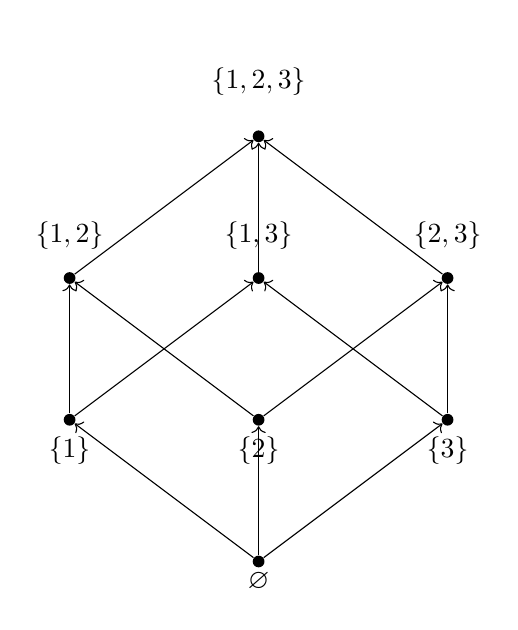
\begin{tikzpicture}[
				scale=1.2,
				every node/.style={circle, fill=black, inner sep=1.5pt}
			]
				\node (empty) at (0,0) {};
				\node (a) at (-2,1.5) {};
				\node (b) at (0,1.5) {};
				\node (c) at (2,1.5) {};
				\node (ab) at (-2,3) {};
				\node (ac) at (0,3) {};
				\node (bc) at (2,3) {};
				\node (abc) at (0,4.5) {};

				\node[draw=none, fill=none, below] at (empty) {$\varnothing$};
				\node[draw=none, fill=none, below] at (a) {$\{1\}$};
				\node[draw=none, fill=none, below] at (b) {$\{2\}$};
				\node[draw=none, fill=none, below] at (c) {$\{3\}$};
				\node[draw=none, fill=none, above] at (ab) {$\{1,2\}$};
				\node[draw=none, fill=none, above] at (ac) {$\{1,3\}$};
				\node[draw=none, fill=none, above] at (bc) {$\{2,3\}$};
				\node[draw=none, fill=none, above] at (abc) {$\{1,2,3\}$};

				\draw[->] (empty) -- (a);
				\draw[->] (empty) -- (b);
				\draw[->] (empty) -- (c);

				\draw[->] (a) -- (ab);
				\draw[->] (a) -- (ac);
				\draw[->] (b) -- (ab);
				\draw[->] (b) -- (bc);
				\draw[->] (c) -- (ac);
				\draw[->] (c) -- (bc);

				\draw[->] (ab) -- (abc);
				\draw[->] (ac) -- (abc);
				\draw[->] (bc) -- (abc);
			\end{tikzpicture}
			\caption{A finite category induced by a partial order.
			Identity morphisms and arrows obtained by composition
			are omitted.}
		\end{figure}
		Composition follows from the transitivity of inclusion:
		if $A \subseteq B \subseteq C$, then
		\begin{equation}
			\iota_{B,C} \circ \iota_{A,B} = \iota_{A,C}.
		\end{equation}
		The object $\varnothing$ is initial, and $\{1,2,3\}$
		is terminal.
	\end{example}

	\begin{definition}[Isomorphism]
		An \textbf{isomorphism} in a category $\mathcal{C}$ is a morphism $f: X \to Y$ such that there exists an inverse morphism $g: Y \to X$ satisfying 
		\begin{equation}
		  f \circ g = 1_Y, \quad g \circ f = 1_X
		\end{equation}
	\end{definition}

	\begin{example}[Isomorphisms]
		Here are some isomorphisms in our familiar categories. 
	  \begin{enumerate}
			\item All bijective functions in $\mathbf{Set}$. 
			\item All group isomorphisms in $\mathbf{Group}$. 
			\item All ring isomorphisms in $\mathbf{Ring}$. 
			\item All field isomorphisms in $\mathbf{Field}$. 
			\item All homeomorphisms in $\mathbf{Top}$. 
			\item All vector space isomorphisms in $\mathbf{Vec}$. 
	  \end{enumerate}
	\end{example}

	\begin{definition}[Notation]
		Given a category $\mathcal{C}$, 
		\begin{enumerate}
			\item $\Ob(\mathcal{C})$ is the collection of all objects in $\mathcal{C}$. 
			\item $\Mor(\mathcal{C})$ is the collection of all morphisms in $\mathcal{C}$. 
			\item $\Hom_{\mathcal{C}}(X, Y)$ is the collection of all morphisms $X \to Y$ in $\mathcal{C}$. 
			\item $\Iso_{\mathcal{C}}(X, Y)$ is the collection of all isomorphisms $X \to Y$ in $\mathcal{C}$. 
			\item $\End_{\mathcal{C}}(X, Y)$ is the collection of all morphisms $X \to X$ in $\mathcal{C}$. 
			\item $\Aut_{\mathcal{C}}(X, Y)$ is the collection of all isomorphisms $X \to X$ in $\mathcal{C}$. 
		\end{enumerate}
		If the context is clear on which category we are working on, we can drop the subscript $\mathcal{C}$. 
	\end{definition}

	Note that these collections, like $\Hom(X, Y)$, may not actually form a set. If they do, we call the category \textit{locally small}. 

	\begin{definition}[Locally Small Category]
		A category $\mathcal{C}$ is \textbf{locally small} if the morphisms between any objects in the category form a set. In this case, we call $\Hom(X, Y)$ a \textit{hom set}. 
	\end{definition}

	\begin{definition}[Subcategory]
		Let $\mathcal C$ be a category. A \textbf{subcategory} $\mathcal D$ of $\mathcal C$ is a category satisfying
		\begin{enumerate}
			\item $\mathrm{Ob}(\mathcal D) \subseteq \mathrm{Ob}(\mathcal C)$.
			\item For all $X, Y \in \mathrm{Ob}(\mathcal D)$,
				\begin{equation}
					\mathrm{Hom}_{\mathcal D}(X,Y)
					\subseteq \mathrm{Hom}_{\mathcal C}(X,Y).
				\end{equation}
			\item For every $X \in \mathrm{Ob}(\mathcal D)$, the identity morphism $\mathrm{id}_X$ belongs to $\mathrm{Hom}_{\mathcal D}(X,X)$.
			\item The composition of morphisms in $\mathcal D$ is the restriction of the composition in $\mathcal C$.
		\end{enumerate}
		A subcategory $\mathcal D$ of $\mathcal C$ is called
		\begin{enumerate}
			\item \textbf{Full} if for every $X,Y \in \mathrm{Ob}(\mathcal D)$,
				\begin{equation}
					\mathrm{Hom}_{\mathcal D}(X,Y)
					= \mathrm{Hom}_{\mathcal C}(X,Y).
				\end{equation}
			\item \textbf{Wide} if $\mathrm{Ob}(\mathcal D) = \mathrm{Ob}(\mathcal C)$.
			\item \textbf{Proper} if $\mathcal D \neq \mathcal C$.
		\end{enumerate}
	\end{definition}

	\begin{example}[Subcategories]
		The following are examples of subcategories.
		\begin{enumerate}
			\item The category $\mathbf{Ab}$ of abelian groups is a full subcategory of $\mathbf{Group}$, since every group homomorphism between abelian groups is also a morphism in $\mathbf{Ab}$.
			\item The category $\mathbf{FinSet}$ of finite sets and functions between them is a full subcategory of $\mathbf{Set}$.
			\item The category $\mathbf{FinVect}_k$ of finite-dimensional vector spaces over a field $k$ and linear transformations between them is a full subcategory of $\mathbf{Vect}_k$.
			\item The category $\mathbf{Haus}$ of Hausdorff topological spaces and continuous maps between them is a full subcategory of $\mathbf{Top}$.
			\item The category $\mathbf{Top}$ with only homeomorphisms as morphisms is a wide subcategory of $\mathbf{Top}$, since it has the same objects but fewer morphisms.
			\item The category of sets with injective functions as morphisms is a wide subcategory of $\mathbf{Set}$, since the composition of injective functions is injective.
			\item The category of sets with bijective functions as morphisms is a wide subcategory of $\mathbf{Set}$.
			\item The category of vector spaces over $k$ with only invertible linear transformations as morphisms is a wide subcategory of $\mathbf{Vect}_k$.
		\end{enumerate}
	\end{example}

\subsection{Functors}

	\begin{definition}[Functor]
		A \textbf{functor} $F: \mathcal{C} \to \mathcal{D}$ between categories $\mathcal{C}$ and $\mathcal{D}$ is a mapping which associates objects $X$ and morphisms $f$ in $\mathcal{C}$ to objects $F(X)$ and morphisms $F(f)$ in $\mathcal{D}$. It must satisfy the properties: 
		\begin{enumerate}
			\item For any objects $X, Y$ in $\mathcal{C}$, $F(f: X \to Y) = F(f): F(X) \to F(Y)$. 
			\item For any morphisms $f, g$ in $\mathcal{C}$, $F(g \circ f) = F(g) \circ F(f)$. 
			\item $F(1_X) = 1_{F(X)}$
		\end{enumerate}

		\[
			\begin{tikzcd}[row sep=large, column sep=large]
				X \arrow[r, mapsto] \arrow[d, "f"'] &
				F(X) \arrow[d, "F(f)"] \\
				Y \arrow[r, mapsto] &
				F(Y)
			\end{tikzcd}
		\]
	\end{definition}

	This allows us to build the category of categories. 

	\begin{example}[$\mathbf{Cat}$]
	  $\mathbf{Cat}$ is the category consisting of categories as its objects and functors as its morphisms. 
	\end{example}

	\begin{definition}[Forgetful Functor]
		A functor $U: \mathcal{C} \to \mathcal{D}$ is a \textbf{forgetful functor} if it sends objects and morphisms of $\mathcal{C}$ to their underlying objects and morphisms in $\mathcal{D}$, discarding some of the additional structure present in $\mathcal{C}$.\footnote{Unlike the functor, there is no single universally accepted definition of what a forgetful functor is.}
	\end{definition}

	\begin{example}[Forgetful Functors]
		The following are examples of forgetful functors.
		\begin{enumerate}
			\item The functor $U: \mathbf{Group} \to \mathbf{Set}$ that associates each group (object in $\mathbf{Group}$) with its underlying set (object in $\mathbf{Set}$) and each group homomorphism (morphism in $\mathbf{Group}$) with its underlying function (morphism in $\mathbf{Set}$).
			\item The functor $U: \mathbf{Ab} \to \mathbf{Group}$ that associates each abelian group with its underlying group and each abelian group homomorphism with the same group homomorphism, forgetting the requirement of commutativity.
			\item The functor $U: \mathbf{Ring} \to \mathbf{Ab}$ that associates each ring with its underlying additive abelian group and each ring homomorphism with its underlying additive group homomorphism, forgetting multiplication.
			\item The functor $U: \mathbf{Ring} \to \mathbf{Set}$ that associates each ring with its underlying set and each ring homomorphism with its underlying function, forgetting both addition and multiplication.
			\item The functor $U: \mathbf{Vect}_k \to \mathbf{Ab}$ that associates each vector space over $k$ with its underlying additive abelian group and each linear transformation with its underlying group homomorphism, forgetting scalar multiplication.
			\item The functor $U: \mathbf{Vect}_k \to \mathbf{Set}$ that associates each vector space over $k$ with its underlying set and each linear transformation with its underlying function, forgetting vector addition and scalar multiplication.
			\item The functor $U: \mathbf{Top} \to \mathbf{Set}$ that associates each topological space with its underlying set and each continuous map with its underlying function, forgetting the topology.
			\item The functor $U: \mathbf{Met} \to \mathbf{Top}$ that associates each metric space with its induced topological space and each continuous map with the same continuous map, forgetting the metric but retaining the induced topology.
			\item The functor $U: \mathbf{Mod}_R \to \mathbf{Ab}$ that associates each left module over a ring $R$ with its underlying additive abelian group and each module homomorphism with its underlying group homomorphism, forgetting scalar multiplication by elements of $R$.
		\end{enumerate}
	\end{example}

	\begin{definition}[Full Functors]
		A functor $F: \mathcal{C} \to \mathcal{D}$ is \textbf{full} when $F_{X, Y}: \Hom_{\mathcal{C}}(X, Y) \to \Hom_{\mathcal{D}} (F(X), F(Y))$ is surjective for any objects $X, Y \in \Ob(C)$. 
	\end{definition}

	\begin{definition}[Faithful Functor]
		A functor $F: \mathcal{C} \to \mathcal{D}$ is \textbf{faithful} when $F_{X, Y}: \Hom_{\mathcal{C}}(X, Y) \to \Hom_{\mathcal{D}} (F(X), F(Y))$ is injective for any objects $X, Y \in \Ob(C)$. 
	\end{definition}

	\begin{definition}[Inclusion Functor]
		Let $\mathcal{D}$ be a subcategory of $\mathcal{C}$. The \textbf{inclusion functor} is the functor
		\begin{equation}
			I: \mathcal D \hookrightarrow \mathcal C
		\end{equation}
		defined by
		\begin{enumerate}
			\item \textit{On objects}. For every $X \in \Ob(\mathcal D)$,
				\begin{equation}
					I(X) = X.
				\end{equation}
			\item \textit{On morphisms}. For every $f \in \Hom_{\mathcal D}(X,Y)$,
				\begin{equation}
					I(f) = f.
				\end{equation}
		\end{enumerate}
		The inclusion functor is always faithful, and it is full if and only if $\mathcal D$ is a full subcategory of $\mathcal C$.
	\end{definition}
	\begin{proof}
	  
	\end{proof}

	\begin{example}
	  Consider the forgetful functor $U: \Group \to \Set$. 
		\begin{enumerate}
			\item $U$ is faithful since for any two groups $G, H \in \Ob(\Group)$, a homomorphism $\varphi: G \to H \in \Mor(\Group)$ is mapped to a unique function $U(\varphi) \in \Mor(\Set)$. Therefore, $U_{G, H}: \Hom_{\Group} (G, H) \to \Hom_{\Set}(U(X), U(Y))$ is injective. 
			\item $U$ is not full since there exists functions in $\Mor(\Set)$ that are not homomorphisms. 
		\end{enumerate}
	\end{example}

	\begin{definition}[Opposite Category]
		Let $\mathcal C$ be a category. The \textbf{opposite category}
		$\mathcal C^{\mathrm{op}}$ is the category obtained by reversing
		the direction of every morphism in $\mathcal C$. More precisely,
		\begin{enumerate}
			\item \textit{Objects}. The objects are the same:
				\begin{equation}
					\Ob(\mathcal C^{\mathrm{op}}) = \Ob(\mathcal C).
				\end{equation}

			\item \textit{Morphisms}. For every pair of objects $X,Y$,
				\begin{equation}
					\Hom_{\mathcal C^{\mathrm{op}}}(X,Y)
					= \Hom_{\mathcal C}(Y,X).
				\end{equation}

			\item \textit{Composition}. If $f: X \to Y$ and
				$g: Y \to Z$ are morphisms in $\mathcal C^{\mathrm{op}}$,
				their composition is defined by
				\begin{equation}
					g \circ_{\mathrm{op}} f = f \circ g,
				\end{equation}
				where the composition on the right is taken in $\mathcal C$.

			\item \textit{Identity}. The identity morphisms are unchanged:
				\begin{equation}
					1_X^{\mathrm{op}} = 1_X.
				\end{equation}
		\end{enumerate}
		In particular,
		\begin{equation}
			(\mathcal C^{\mathrm{op}})^{\mathrm{op}} = \mathcal C.
		\end{equation}
	\end{definition}

	\begin{example}[Opposite Categories]
		The following are examples of opposite categories.
		\begin{enumerate}
			\item Let $\mathcal C$ be the category
				\begin{equation}
					\begin{tikzcd}[column sep=large]
						X \arrow[r, "f"] & Y \arrow[r, "g"] & Z
					\end{tikzcd}
				\end{equation}
				together with identities and compositions. Then
				$\mathcal C^{\mathrm{op}}$ has the reversed arrows
				\begin{equation}
					\begin{tikzcd}[column sep=large]
						X & Y \arrow[l, "f^{\mathrm{op}}"']
							& Z \arrow[l, "g^{\mathrm{op}}"']
					\end{tikzcd}
				\end{equation}
				satisfying
				\begin{equation}
					f^{\mathrm{op}} \circ g^{\mathrm{op}}
					= (g \circ f)^{\mathrm{op}}.
				\end{equation}

			\item Every partially ordered set $(P,\leq)$ can be
				regarded as a category in which there exists a unique
				morphism $x \to y$ if and only if $x \leq y$.
				Its opposite category corresponds to the reversed
				partial order $(P,\geq)$.

			\item An object $I$ is initial in $\mathcal C$ if and
				only if it is terminal in $\mathcal C^{\mathrm{op}}$.
				Similarly, terminal objects in $\mathcal C$ are
				initial objects in $\mathcal C^{\mathrm{op}}$.
		\end{enumerate}
	\end{example}

	\begin{definition}[Covariant and Contravariant Functors]
		Let $\mathcal C$ and $\mathcal D$ be categories.
		\begin{enumerate}
			\item A \textbf{covariant functor}
				$F: \mathcal C \to \mathcal D$ preserves the
				direction of morphisms. That is, for every
				morphism $f: X \to Y$ in $\mathcal C$,
				\begin{equation}
					F(f): F(X) \to F(Y).
				\end{equation}

			\item A \textbf{contravariant functor}
				$F: \mathcal C \to \mathcal D$ reverses the
				direction of morphisms. That is, for every
				morphism $f: X \to Y$ in $\mathcal C$,
				\begin{equation}
					F(f): F(Y) \to F(X).
				\end{equation}
				It satisfies
				\begin{equation}
					F(1_X) = 1_{F(X)}, \qquad
					F(g \circ f) = F(f) \circ F(g)
				\end{equation}
				for every pair of composable morphisms $f,g$.
		\end{enumerate}

		Equivalently, a contravariant functor
		$F: \mathcal C \to \mathcal D$ is an ordinary
		covariant functor
		\begin{equation}
			F: \mathcal C^{\mathrm{op}} \to \mathcal D.
		\end{equation}
	\end{definition}

	\begin{example}[Covariant and Contravariant Functors]
		The following are examples.
		\begin{enumerate}
			\item The forgetful functor
				$U: \Group \to \Set$ is covariant, since
				a homomorphism $f: G \to H$ is mapped
				to a function $U(f): U(G) \to U(H)$.

			\item The dual space construction is a contravariant
				functor
				\begin{equation}
					(-)^*: \Vect_k \to \Vect_k.
				\end{equation}
				It maps every vector space $V$ to its dual
				\begin{equation}
					V^* = \Hom_k(V,k)
				\end{equation}
				and every linear transformation $T: V \to W$
				to its dual transformation
				\begin{equation}
					T^*: W^* \to V^*, \qquad
					\varphi \mapsto \varphi \circ T.
				\end{equation}
				This reverses the direction of morphisms,
				as depicted by
				\begin{equation}
					\begin{tikzcd}[column sep=huge, row sep=large]
						V \arrow[r, "T"] & W \\
						V^* & W^* \arrow[l, "T^*"']
					\end{tikzcd}
				\end{equation}
				Moreover,
				\begin{equation}
					(S \circ T)^* = T^* \circ S^*.
				\end{equation}

			\item The power set construction defines a
				contravariant functor
				\begin{equation}
					\mathcal P: \Set \to \Set
				\end{equation}
				by associating each set $X$ with its power
				set $\mathcal P(X)$, and each function
				$f: X \to Y$ with the inverse-image function
				\begin{equation}
					f^{-1}: \mathcal P(Y) \to \mathcal P(X).
				\end{equation}
				Since
				\begin{equation}
					(g \circ f)^{-1} = f^{-1} \circ g^{-1},
				\end{equation}
				composition is reversed.
		\end{enumerate}
	\end{example}

	\begin{definition}[Hom-Functors]
		Let $\mathcal C$ be a locally small category,
		and fix an object $A \in \Ob(\mathcal C)$.
		There are two canonical \textbf{Hom-functors}.
		\begin{enumerate}
			\item \textit{Covariant Hom-Functor}. The functor
				\begin{equation}
					H_A = \Hom_{\mathcal C}(A,-):
					\mathcal C \to \Set
				\end{equation}
				is defined on objects by
				\begin{equation}
					H_A(X) = \Hom_{\mathcal C}(A,X)
				\end{equation}
				and on morphisms $f: X \to Y$ by
				\begin{equation}
					H_A(f): \Hom_{\mathcal C}(A,X)
					\to \Hom_{\mathcal C}(A,Y),
					\qquad g \mapsto f \circ g.
				\end{equation}
				Thus, $H_A(f)$ acts by postcomposition with $f$.
				\begin{equation}
					\begin{tikzcd}[column sep=large]
						A \arrow[r, "g"]
							\arrow[rr, bend right=25, "f\circ g"'] &
						X \arrow[r, "f"] & Y
					\end{tikzcd}
				\end{equation}

			\item \textit{Contravariant Hom-Functor}. The functor
				\begin{equation}
					H^A = \Hom_{\mathcal C}(-,A):
					\mathcal C^{\mathrm{op}} \to \Set
				\end{equation}
				is defined on objects by
				\begin{equation}
					H^A(X) = \Hom_{\mathcal C}(X,A)
				\end{equation}
				and on morphisms $f: X \to Y$ in $\mathcal C$ by
				\begin{equation}
					H^A(f): \Hom_{\mathcal C}(Y,A)
					\to \Hom_{\mathcal C}(X,A),
					\qquad g \mapsto g \circ f.
				\end{equation}
				Thus, $H^A(f)$ acts by precomposition with $f$.
				\begin{equation}
					\begin{tikzcd}[column sep=large]
						X \arrow[r, "f"]
							\arrow[rr, bend right=25, "g\circ f"'] &
						Y \arrow[r, "g"] & A
					\end{tikzcd}
				\end{equation}
		\end{enumerate}

		More generally, the \textbf{Hom-bifunctor} is
		\begin{equation}
			\Hom_{\mathcal C}(-,-):
			\mathcal C^{\mathrm{op}} \times \mathcal C
			\to \Set,
		\end{equation}
		which is contravariant in its first argument
		and covariant in its second argument.
	\end{definition}

	\begin{example}[Hom-Functors]
		The following are examples of Hom-functors.
		\begin{enumerate}
			\item In $\Set$, fixing a set $A$ gives the
				covariant Hom-functor
				\begin{equation}
					H_A(X) = \Hom_{\Set}(A,X).
				\end{equation}
				For every function $f: X \to Y$, it maps
				each function $g: A \to X$ to $f \circ g$.

			\item In $\Group$, fixing $A = \mathbb Z$ gives
				\begin{equation}
					H_{\mathbb Z}(G)
					= \Hom_{\Group}(\mathbb Z,G).
				\end{equation}
				Every homomorphism $\varphi: \mathbb Z \to G$
				is uniquely determined by $\varphi(1)$.
				Therefore, there is a natural bijection
				\begin{equation}
					H_{\mathbb Z}(G) \cong U(G),
					\qquad \varphi \mapsto \varphi(1),
				\end{equation}
				where $U: \Group \to \Set$ is the forgetful
				functor. Hence,
				\begin{equation}
					H_{\mathbb Z} \cong U
				\end{equation}
				as functors.

			\item In $\Vect_k$, fixing $A=k$ gives the
				covariant Hom-functor
				\begin{equation}
					H_k(V) = \Hom_k(k,V).
				\end{equation}
				Every linear transformation $T:k\to V$
				is uniquely determined by $T(1)$.
				Therefore,
				\begin{equation}
					\Hom_k(k,V) \cong V
				\end{equation}
				naturally as sets.

			\item In $\Vect_k$, the dual space construction
				is the contravariant Hom-functor
				\begin{equation}
					(-)^* = \Hom_k(-,k).
				\end{equation}
				It sends a linear transformation $T:V\to W$
				to the dual map $T^*:W^*\to V^*$.
		\end{enumerate}
	\end{example}

\subsection{Natural Transformations}

	So far, general categories and functors are pretty abstract, so we would like to represent them in some category we are familiar with, say $\Set$. Let $\mathcal{C}$ be a locally small category and choose an object $A \in \Ob(\mathcal{C})$. Now consider the functor 
	\begin{equation}
		H_A: \mathcal{C} \to \Set
	\end{equation}
	We must define its actions on objects and morphisms in $\mathcal{C}$. 
	\begin{enumerate}
	  \item Given an object $X \in \Ob(\mathcal{C})$, we define 
			\begin{equation}
				H_A (X) \coloneqq \Hom_{\mathcal{C}}(A, X)
			\end{equation}
			which is viable since $\Hom_{\mathcal{C}}(A, X) = \{g : A \to X\}$ is a set, i.e. an object in $\Set$.  

		\item Let $f: X \to Y$ be a morphism in $\mathcal{C}$. To define its actions on functions, note that by definition of a functor, we must have $H_A (f): H_A (X) \to H_A(Y)$, that is
			\begin{equation}
				H_A (f): \Hom_{\mathcal{C}}(A, X) \to \Hom_{\mathcal{C}} (A, Y)
			\end{equation}
			$H_A (f)$ should be a morphism in $\Set$, i.e. a function, and this function will take morphisms $g: A \to X$ and must output a morphism $h: A \to Y$. This should give us a hint on how to define $H_A(f)$. Recall that if we have a morphisms $g: A \to X$ and $f: X \to Y$ in a category, we must have the composition $f \circ g: A \to Y$. Therefore, we can define 
			\begin{equation}
			  H_A (f)(g) = f \circ g
			\end{equation}
			aka postcomposition of $g$ with $f$. 
	\end{enumerate}

	\begin{center}
		\begin{tikzcd}[column sep=large]
			A \arrow[r,"g"] \arrow[rr,bend right=25,"f\circ g"'] &
			X \arrow[r,"f"] & Y
		\end{tikzcd}
	\end{center}
	
	Therefore, we have transferred all objects and morphisms in $\mathcal{C}$ to objects and morphisms in $\Set$. We can consider 
	\begin{enumerate}
		\item objects $X \in \Ob(\mathcal{C})$ as sets $\Hom_{\mathcal{C}}(A, X) = \{g : A \to X\}$.  
		\item morphisms $f: X \to Y$ as functions $H_A (f) : H_A (X) \to H_A (Y)$. 
		\item compositions $f \circ g$ as compositions of functions $H_A (f) \circ H_A (g)$. 
	\end{enumerate}

	\begin{definition}[Functor Category]
		Let $\mathcal C$ and $\mathcal D$ be categories.
		The \textbf{functor category}, denoted
		$[\mathcal C,\mathcal D]$, is the category defined by
		\begin{enumerate}
			\item \textit{Objects}. Functors $F:\mathcal C\to\mathcal D$.

			\item \textit{Morphisms}. Natural transformations
				$\eta:F\Rightarrow G$ between functors.

			\item \textit{Composition}. Given natural transformations
				$\eta:F\Rightarrow G$ and $\theta:G\Rightarrow H$,
				their composition $\theta\circ\eta:F\Rightarrow H$
				is defined componentwise by
				\begin{equation}
					(\theta\circ\eta)_X=\theta_X\circ\eta_X.
				\end{equation}

			\item \textit{Identity}. For every functor $F$, the
				identity natural transformation $1_F:F\Rightarrow F$
				is defined by
				\begin{equation}
					(1_F)_X=1_{F(X)}.
				\end{equation}
		\end{enumerate}
		When size conditions are appropriate, these data form
		a category. In particular, if $\mathcal C$ is small
		and $\mathcal D$ is locally small, the functor category
		is locally small.

		The isomorphisms in $[\mathcal C,\mathcal D]$ are
		precisely the natural isomorphisms.
	\end{definition}

	\begin{example}[Functor Categories]
		The following are examples of functor categories.
		\begin{enumerate}
			\item The category $[\mathcal C,\Set]$ has set-valued
				functors as objects and natural transformations
				between them as morphisms.

			\item The category $[\mathcal C^{\mathrm{op}},\Set]$
				has contravariant set-valued functors as objects
				and natural transformations between them as
				morphisms. Its objects are called
				\textbf{presheaves} on $\mathcal C$.

			\item If $\mathcal C$ is the category with two objects
				$0,1$ and one nonidentity morphism $0\to1$,
				then an object of $[\mathcal C,\Set]$ is a function
				$f:X\to Y$. A morphism between two such objects
				$f:X\to Y$ and $g:X'\to Y'$ is a pair of functions
				$a:X\to X'$ and $b:Y\to Y'$ satisfying
				\begin{equation}
					g\circ a=b\circ f.
				\end{equation}
				Equivalently, it is a commutative square
				\begin{equation}
					\begin{tikzcd}[row sep=large, column sep=large]
						X \arrow[r, "a"] \arrow[d, "f"'] &
						X' \arrow[d, "g"] \\
						Y \arrow[r, "b"'] & Y'
					\end{tikzcd}
				\end{equation}
				Thus, this functor category is the arrow
				category of $\Set$.
		\end{enumerate}
	\end{example}


	\begin{definition}[Natural Transformation]
		For two functors $F, G: \mathcal{C} \to \mathcal{D}$, a \textbf{natural transformation} is a family of morphisms $\eta = (\eta_X)_{X \in \Ob(\mathcal{C})}$ where $\eta_X \in \Hom_{\mathcal{D}}(F(X), G(X))$.\footnote{$\eta$ is a morphism in the \textit{functor category} $[\mathcal{C}, \mathcal{D}]$, where the objects are functors and morphisms are natural transformations.} It must satisfy the following properties: 
		\begin{enumerate}
			\item It assigns every object $X \in \Ob(\mathcal{C})$ to a morphism in $\mathcal{D}$. 
				\begin{equation}
				  X \mapsto \eta_X : F(X) \to G(X)
				\end{equation}
			\item The assignments above much be such that for any $f: X \to Y$ in $\mathcal{C}$, we have 
				\begin{equation}
				  \eta_Y \circ F(f) = G(f) \circ \eta_X
				\end{equation}
				depicted through the commutative diagram. 

				\[
					X \xrightarrow{\hspace{1cm}} Y
					\qquad \rightsquigarrow \qquad
					\begin{tikzcd}[column sep=large, row sep=large]
						F(X) \arrow[r, "\eta_X"] \arrow[d, "F(f)"']
						& G(X) \arrow[d, "G(f)"] \\
						F(Y) \arrow[r, "\eta_Y"']
						& G(Y)
					\end{tikzcd}
				\]
		\end{enumerate}
	\end{definition}

	\begin{example}[$\Group$ ]
		Consider $\mathcal{C} = \Group$, and let us choose $A = \mathbb{Z}$. Then, we can construct the functor by first defining its action on groups $H_{\mathbb{Z}} : \Group \to \Set$. 
		\begin{equation}
			H_{\mathbb{Z}}(G) = \Hom_{\Group}(\mathbb{Z}, G) = \{\varphi : \mathbb{Z} \to G \colon \varphi \text{ is a group homomorphism}\}
		\end{equation}
		But this homomorphism is entirely determined by $\varphi(1)$ since $\varphi(n) = \varphi(1)^n$. Moreoever, every element $g \in G$ determines a unique group homomorphism, so we have a natural bijection (as sets) 
		\begin{equation}
			H_{\mathbb{Z}}(G) \cong G, \quad \varphi_g \cong g
		\end{equation}
		where $\varphi_g (1) = g$. Now consider a group homomorphism $f: G \to K$. Then, we can define 
		\begin{equation}
			H_{\mathbb{Z}}(f) : \Hom_{\Group}(\mathbb{Z}, G) \to \Hom_{\Group}(G, K), \quad H_{\mathbb{Z}}(f)(\varphi_g) \coloneqq f \circ \varphi_g
		\end{equation}
		But note that $H_{\mathbb{Z}} (f) (\varphi_g)(1) = (f \circ \varphi_g)(1) = f(\varphi_g(1)) = f(g)$. Therefore, $H_{\mathbb{Z}}(f)$ behaves exactly like the underlying function $f$! That is, given $H_{\mathbb{Z}} (f)$, 
		\begin{equation}
			g \mapsto H_{\mathbb{Z}} (f)(g)(1) = f(g)
		\end{equation}
		So, groups are mapped to their underlying sets, and group homomorphisms are mapped to functions that---when evaluated at $g$ and then evaluated at $1$---gives the action of $f$ on $g$. 
	\end{example}

	But this may not capture the entire category. For an arbitrary choice of $A$, the functor $H_A: \mathcal{C} \to \Set$ might lose information. 

	\begin{example}
		If $\mathcal{C} = \Group$ and $A$ is the trivial group, then $\Hom_{\Group}(A, G)$ contains exactly 1 homomorphism for every group $G$. Consequently, $H_A$ sends every group to a singleton set and every group homomorphism to the unique function between singleton sets. 
	\end{example}

	\begin{definition}[Natural Isomorphism]
		Let $F,G:\mathcal C\to\mathcal D$ be functors.
		A natural transformation $\eta:F\Rightarrow G$ is called
		a \textbf{natural isomorphism} if every component
		\begin{equation}
			\eta_X:F(X)\to G(X)
		\end{equation}
		is an isomorphism in $\mathcal D$.

		Equivalently, there exists a natural transformation
		$\eta^{-1}:G\Rightarrow F$ satisfying
		\begin{equation}
			\eta_X^{-1}\circ\eta_X=1_{F(X)},\qquad
			\eta_X\circ\eta_X^{-1}=1_{G(X)}
		\end{equation}
		for every $X\in\Ob(\mathcal C)$.

		In this case, $F$ and $G$ are said to be
		\textbf{naturally isomorphic}, denoted
		\begin{equation}
			F\cong G.
		\end{equation}
	\end{definition}

	\begin{example}[Natural Isomorphism]
		Consider the double dual functor
		\begin{equation}
			(-)^{**}:\FinVect_k\to\FinVect_k.
		\end{equation}
		For every finite-dimensional vector space $V$, define
		\begin{equation}
			\eta_V:V\to V^{**},\qquad
			\eta_V(v)(\varphi)=\varphi(v)
		\end{equation}
		for every $\varphi\in V^*$.

		Each $\eta_V$ is a vector space isomorphism. Moreover,
		for every linear transformation $T:V\to W$,
		\begin{equation}
			\eta_W\circ T=T^{**}\circ\eta_V.
		\end{equation}
		This is represented by the commutative diagram
		\begin{equation}
			\begin{tikzcd}[row sep=large, column sep=large]
				V \arrow[r, "\eta_V"] \arrow[d, "T"'] &
				V^{**} \arrow[d, "T^{**}"] \\
				W \arrow[r, "\eta_W"'] & W^{**}
			\end{tikzcd}
		\end{equation}
		Therefore, the identity functor and double dual functor
		are naturally isomorphic:
		\begin{equation}
			1_{\FinVect_k}\cong(-)^{**}.
		\end{equation}
	\end{example}

\subsection{Universal Properties}

  A \textbf{universal property} characterizes a mathematical object through its relationships with other objects and morphisms, rather than through its internal construction. The central idea is that universal properties can often be expressed as initial or terminal objects in suitably constructed categories.

  \begin{definition}[Initial, Terminal, and Universal Objects]
    Let $\mathcal C$ be a category. 
		\begin{enumerate}
		  \item An object $I \in \Ob(\mathcal C)$ is called an \textbf{initial object} if for every object $X \in \Ob(\mathcal C)$, there exists a unique morphism $f: I \to X$. 
				\begin{equation}
					\begin{tikzcd}[column sep=large, row sep=large]
						& I \arrow[dl, "!"'] \arrow[dr, "!"] & \\
						X & & Y
					\end{tikzcd}
				\end{equation}

			\item An object $T \in \Ob(\mathcal C)$ is called a \textbf{terminal object} if for every object $X \in \Ob(\mathcal C)$, there exists a unique morphism $f: X \to T$. 
				\begin{equation}
					\begin{tikzcd}[column sep=large, row sep=large]
						X \arrow[dr, "!"'] & & Y \arrow[dl, "!"] \\
						& T &
					\end{tikzcd}
				\end{equation}
				
			\item An object $U \in \Ob(\mathcal{C})$ is called a \textbf{universal object} if it is an initial or terminal object. 
		\end{enumerate}
		If an initial or terminal object exists in a category $\mathcal{C}$, it is unique up to unique isomorphism. 
  \end{definition}
  \begin{proof}
    Suppose $I$ and $I'$ are both initial objects. By initiality, there exist unique morphisms
    \begin{equation}
      f: I \to I', \qquad g: I' \to I.
    \end{equation}
    Then $g \circ f: I \to I$ is an endomorphism of $I$. Since $I$ is initial, there exists exactly one such endomorphism, which must be $1_I$. Therefore,
    \begin{equation}
      g \circ f = 1_I.
    \end{equation}
    Similarly, $f \circ g = 1_{I'}$, so $f$ and $g$ are inverses. Hence $I \cong I'$. The isomorphism is unique by initiality. The proof for terminal objects is analogous to that of initial objects. 
  \end{proof}

  \begin{example}[Initial and Terminal Objects]
    The following are examples of initial and terminal objects.
    \begin{enumerate}
      \item In $\Set$, the empty set $\varnothing$ is initial, since there exists a unique function $\varnothing \to X$ for every set $X$. Any singleton set $\{*\}$ is terminal, since there exists a unique function $X \to \{*\}$ for every set $X$.

      \item In $\Group$, the trivial group $\{e\}$ is both initial and terminal, since there exists a unique group homomorphism $\{e\} \to G$ and a unique group homomorphism $G \to \{e\}$ for every group $G$.

      \item In $\Vect_k$, the zero vector space $\{0\}$ is both initial and terminal, since there exists a unique linear transformation from or into $\{0\}$.

      \item In $\Top$, the empty topological space is initial, while any singleton topological space is terminal.
    \end{enumerate}
    An object that is both initial and terminal is called a \textbf{zero object}.
  \end{example}

	Suppose a mathematical problem determines a category $\mathcal D$ whose objects represent candidate solutions and whose morphisms represent compatible maps between solutions. Thus, to formulate a universal property, we can construct a category of candidate solutions and characterize the desired construction as an initial or terminal object in that category.

  \begin{example}[Cartesian Product as Terminal Universal Object]
		Let $A, B$ be sets. For any functions $f: X \to A, g: X \to B$, we know from the \hyperref[st-thm:universal_cartesian]{universal property of Cartesian products} that there exists a unique function $(f, g): X \to A \times B$ satisfying $f = \pi_A \circ (f, g)$ and $g = \pi_B \circ (f, g)$. 
		
    \begin{equation}
      \begin{tikzcd}[column sep=large, row sep=large]
        & X \arrow[dl, "f"'] \arrow[dr, "g"]
            \arrow[d, dashed, "{\exists!\,\langle f,g\rangle}" description] & \\
        A & A\times B \arrow[l, "\pi_A"]
            \arrow[r, "\pi_B"'] & B
      \end{tikzcd}
    \end{equation}

		We wish to restate this in categorical terms, and show their equivalence. 

		\begin{enumerate}
		  \item $(\rightarrow)$. Since the result above is true, Consider the category $\mathcal{P}_{A, B}$ consisting of objects $(X, f: X \to A, g: X \to B)$ and morphisms $h: (X, f, g) \to (Y, f^\prime, g^\prime)$---which are functions $h: X \to Y$---satisfying 
				\begin{equation}
					f^\prime \circ h = f, \quad  g^\prime \circ h = g
				\end{equation}
				We claim that $(A \times B, \pi_A: A \times B \to A, \pi_B: A \times B \to B)$ is a terminal object. Let $(X, f, g)$ be any object in $\mathcal{P}_{A, B}$. Then, we must find a morphism $h: X \to A \times B$ s.t. 
				\begin{equation}
					\pi_A \circ h = f, \quad \pi_B \circ h = g
				\end{equation}
				By the universal property of the Cartesian product, there exists a unique function $h = (f,g)$ satisfying these equations. Hence, there exists exactly one morphism
				\begin{equation}
					(X,f,g) \to (A\times B,\pi_A,\pi_B)
				\end{equation}
				in $\mathcal P_{A,B}$, proving that $(A\times B,\pi_A,\pi_B)$ is terminal.

			\item $(\leftarrow)$ now assume that $(A \times B, \pi_A, \pi_B)$ is a terminal object. Then, for any object $(X, f, g)$ there exists a unique morphism $h: (X, f, g) \to (A \times B, \pi_A, \pi_B)$ satisfying 
				\begin{equation}
				  \pi_A \circ h = f, \quad \pi_B \circ h = g
				\end{equation}
				We have proven existence and uniqueness, so we are done. Indeed, we can easily check that the function $h(x) = (f(x), g(x)) = (f, g)(x)$ works, and it must be unique. Therefore, for functions $f: X \to A, g: X \to B$, there exists a unique $h = (f, g) : X \to A \times B$ satisfying 
				\begin{equation}
				  \pi_A \circ (f, g) = f, \quad \pi_B \circ (f, g) = g
				\end{equation}
		\end{enumerate}
		Therefore, we have reformulated our theorem with the equivalent statement that $(A \times B, \pi_A, \pi_B)$ is terminal. 
  \end{example}

  \begin{example}[Quotient Vector Spaces as Initial Universal Objects]
		Let $V$ be a vector space over $\mathbb{F}$, and let $W$ be a subspace. Then, for any linear map $f: V \to Z$ satisfying $W \subset \ker(f)$, by the \hyperref[lin-thm:universal_quotient]{universal property of quotient spaces}, there exists a unique linear map $\overline{f}: V/W \to Z$ satisfying $f = \overline{f} \circ \pi$, where $\pi: V \to V/W$ is the canonical projection. 

    \begin{equation}
      \begin{tikzcd}[column sep=large, row sep=large]
        V \arrow[r, "\pi"] \arrow[dr, "f"'] &
        V/W \arrow[d, dashed, "\exists!\overline f"] \\
        & Z
      \end{tikzcd}
    \end{equation}

		We wish to restate this in categorical terms and show their equivalence. 
		\begin{enumerate}
			\item $(\rightarrow)$. Since the above result is true, consider the category $\mathcal{Q}_W$ consisting of objects $(Z, f: V \to Z)$---where $Z$ is a vector space and $f$ is linear with $W \subset \ker(f)$---and morphisms $h: (Z, f) \to (Z^\prime, f^\prime)$---which are linear maps $h: Z \to Z^\prime$---satisfying 
				\begin{equation}
				  h \circ f = f^\prime
				\end{equation}
				We claim that $(V/W, \pi)$ is an initial object in $\mathcal{Q}_W$. Let $(Z, f)$ be any object in $\mathcal{Q}_W$. Then, we must find a morphism $h: V/W \to Z$ such that 
				\begin{equation}
				  h \circ \pi = f 
				\end{equation}
				But we have just proved that $h = \overline{f}$ is the unique map, so $(V/W, \pi)$ must be initial. 

			\item $(\leftarrow)$. Now assume that $(V/W, \pi)$ is an initial object. Then, for any object $(Z, f)$, there exists a unique morphism $h: (V/W, \pi) \to (Z, f)$ satisfying 
				\begin{equation}
				  h \circ \pi = f
				\end{equation}
				Indeed, since $\pi(v) = [v]$, we must have $h([v]) = h(\pi(v)) = f(v)$---which is well-defined since $W \subset \ker(f)$--- satisfies this property, so it must be the unique morphism. Therefore, for any linear map $f: V \to Z$ with $W \subset \ker(f)$, there exists a unique linear map $h = \overline{f}: V/W \to Z$ such that $f = \overline{f} \circ \pi$. 
		\end{enumerate}
    Therefore, the universal property of the quotient space is precisely the initiality of $(V/W,\pi)$ in $\mathcal Q_W$.
  \end{example}

	\begin{example}[Quotient Topological Spaces as Initial Universal Objects]
		Let $X$ be a topological space equipped with an equivalence relation $\sim$. Then, from the \hyperref[pst-thm:universal_quotient]{universal property of quotient spaces}, we know that for any topological space $Y$ and continuous map $f: X \to Y$ satisfying $x \sim x^\prime \implies f(x) = f(x^\prime)$, there exists a unique continuous map $\overline{f}: X/{\sim} \to Y$ satisfying $f = \overline{f} \circ q$, where $q: X \to X/{\sim}$ is the canonical quotient map and $X/{\sim}$ is equipped with the quotient topology.

		\begin{equation}
			\begin{tikzcd}[column sep=large, row sep=large]
				X \arrow[r, "q"] \arrow[dr, "f"'] &
				X/{\sim} \arrow[d, dashed, "\exists!\overline f"] \\
				& Y
			\end{tikzcd}
		\end{equation}

		We wish to restate this in categorical terms and show their equivalence.
		\begin{enumerate}
			\item $(\rightarrow)$. Since the above result is true, consider the category $\mathcal{Q}_{\sim}$ consisting of objects $(Y, f: X \to Y)$---where $Y$ is a topological space and $f$ is continuous with $x \sim x^\prime \implies f(x) = f(x^\prime)$---and morphisms $h: (Y, f) \to (Y^\prime, f^\prime)$---which are continuous maps $h: Y \to Y^\prime$---satisfying
				\begin{equation}
					h \circ f = f^\prime.
				\end{equation}
				We claim that $(X/{\sim}, q)$ is an initial object in $\mathcal{Q}_{\sim}$. Let $(Y, f)$ be any object in $\mathcal{Q}_{\sim}$. Then, we must find a morphism $h: X/{\sim} \to Y$ such that
				\begin{equation}
					h \circ q = f.
				\end{equation}
				By the universal property of the quotient topological space, there exists a unique continuous map $h = \overline{f}$ satisfying this equation. Hence, there exists exactly one morphism
				\begin{equation}
					(X/{\sim}, q) \to (Y, f)
				\end{equation}
				in $\mathcal{Q}_{\sim}$, proving that $(X/{\sim}, q)$ is initial.

			\item $(\leftarrow)$. Now assume that $(X/{\sim}, q)$ is an initial object. Then, for any object $(Y, f)$, there exists a unique morphism $h: (X/{\sim}, q) \to (Y, f)$ satisfying
				\begin{equation}
					h \circ q = f.
				\end{equation}
				We have proven existence and uniqueness, so we are done. Indeed, since $q(x) = [x]$, we must have
				\begin{equation}
					h([x]) = h(q(x)) = f(x).
				\end{equation}
				Therefore, for any continuous map $f: X \to Y$ constant on equivalence classes, there exists a unique continuous map $h = \overline{f}: X/{\sim} \to Y$ satisfying
				\begin{equation}
					f = \overline{f} \circ q.
				\end{equation}
		\end{enumerate}
		Therefore, the universal property of the quotient topological space is precisely the initiality of $(X/{\sim},q)$ in $\mathcal{Q}_{\sim}$.
	\end{example}

	\begin{example}[Tensor Products as Initial Universal Objects]
		Let $V, W$ be vector spaces over $\mathbb{F}$. We know from \hyperref[lin-thm:universal_tensor]{the universal property of tensor products} that for any vector space $Z$ and bilinear map $b: V \times W \to Z$, there exists a unique linear map $\widetilde{b}: V \otimes W \to Z$ satisfying $b = \widetilde{b} \circ \tau$, where $\tau: V \times W \to V \otimes W$ is the canonical bilinear map defined as the linear extension of $\tau(v,w) = v \otimes w$.

		\begin{equation}
			\begin{tikzcd}[column sep=large, row sep=large]
				V \times W \arrow[r, "\tau"] \arrow[dr, "b"'] &
				V \otimes W \arrow[d, dashed, "\exists!\widetilde b"] \\
				& Z
			\end{tikzcd}
		\end{equation}

		We wish to restate this in categorical terms and show their equivalence.
		\begin{enumerate}
			\item $(\rightarrow)$. Since the above result is true, consider the category $\mathcal{T}_{V,W}$ consisting of objects $(Z, b: V \times W \to Z)$---where $Z$ is a vector space and $b$ is bilinear---and morphisms $h: (Z, b) \to (Z^\prime, b^\prime)$---which are linear maps $h: Z \to Z^\prime$---satisfying
				\begin{equation}
					h \circ b = b^\prime.
				\end{equation}
				We claim that $(V \otimes W, \tau)$ is an initial object in $\mathcal{T}_{V,W}$. Let $(Z, b)$ be any object in $\mathcal{T}_{V,W}$. Then, we must find a morphism $h: V \otimes W \to Z$ such that
				\begin{equation}
					h \circ \tau = b.
				\end{equation}
				By the universal property of the tensor product, there exists a unique linear map $h = \widetilde{b}$ satisfying this equation. Hence, there exists exactly one morphism
				\begin{equation}
					(V \otimes W, \tau) \to (Z, b)
				\end{equation}
				in $\mathcal{T}_{V,W}$, proving that $(V \otimes W, \tau)$ is initial.

			\item $(\leftarrow)$. Now assume that $(V \otimes W, \tau)$ is an initial object. Then, for any object $(Z, b)$, there exists a unique morphism $h: (V \otimes W, \tau) \to (Z, b)$ satisfying
				\begin{equation}
					h \circ \tau = b.
				\end{equation}
				We have proven existence and uniqueness, so we are done. Indeed, since $\tau(v,w) = v \otimes w$, we must have
				\begin{equation}
					h(v \otimes w) = h(\tau(v,w)) = b(v,w).
				\end{equation}
				Therefore, for any bilinear map $b: V \times W \to Z$, there exists a unique linear map $h = \widetilde{b}: V \otimes W \to Z$ satisfying
				\begin{equation}
					b = \widetilde{b} \circ \tau.
				\end{equation}
		\end{enumerate}
		Therefore, the universal property of the tensor product is precisely the initiality of $(V \otimes W,\tau)$ in $\mathcal{T}_{V,W}$.
	\end{example}

  These examples illustrate the same underlying principle: a mathematical construction is characterized by the existence of a unique compatible morphism between candidate solutions.



\end{document}

